\chapter{把研究内容变成一份绘图任务书}


研究者往往能够用几分钟向同事讲清一个课题，却难以用几句话告诉绘图工具应该画什么。口头交流允许随时补充前提，也能借助双方共有的背景。绘图输入则需要把这些隐含内容写出来。

例如，“画一张通路图，体现上游激活、下游作用以及抑制剂干预”，听起来已经像一个完整任务。但上游是谁？激活的是哪个对象？下游作用是观测结果还是推测？抑制剂影响哪个环节？这些问题没有答案时，生成图片只能自行填充结构。

绘图任务书的作用，是把作者掌握的研究内容变成一份可以执行和检查的说明。

\section{任务书与提示词各管什么}

任务书记录你希望表达的内容及其依据。提示词则针对一次操作，把任务书中的相关部分交给工具。它们可以非常接近，也可能随着操作阶段不同而有明显差别。

初次生成需要解释对象、关系和布局。调整颜色时，可能只需要给出新的颜色分工及保持不变的内容。补写图注时，则需要图和相应的文字说明。任务书帮助你判断这些局部操作是否仍然服务于同一个目标。

因此，不必为了写出一个“万能提示词”把所有要求塞进一段长文字。先把任务书写清，再为具体步骤选取信息。后续修改涉及科学内容时，也应更新任务书，避免旧版本的说明继续驱动新图。

\section{用七个问题构成任务书}

配套模板有十个填写项。实际思考时，可以用下面七个问题组织它们。

\textbf{第一，给谁看，在哪里用？} 同一研究可以为领域同行、跨学科评审或课堂读者制作不同图片。用途还决定了最终观看尺寸。写“论文结果部分，供了解基本方法的同行阅读”，比只写“论文风格”更能影响取舍。

\textbf{第二，主要回答什么问题？} 用一句话写出图的中心任务。如果句子里连续出现多个“以及”，试着把它拆成几个面板，并为每个面板分配一个问题。

\textbf{第三，依据哪些材料？} 记录文件名、工作表、实验记录或文献位置。材料不是越多越好，而是要能够支持这张图里的每个重要陈述。不同版本的结果不要混在同一个输入中。

\textbf{第四，必须出现哪些对象和关系？} 列出对象后，还要说明它们的对应关系、方向、分组与空间位置。数据图中的“同一对象两次测量”也是关系，需要与机制图中的箭头一样明确。

\textbf{第五，哪些是事实，哪些是解释？} 观测、推断和假设需要保持各自的身份。任务书中写明不确定性，图中再用标签或约定线型表达，并在图例中解释。不能把一条没有证据的关系交给工具自行决定。

\textbf{第六，希望怎样呈现？} 此时再确定图型、阅读方向、面板、颜色角色和标签语言。给出能帮助理解内容的约束，避免用大量形容词代替具体布局。

\textbf{第七，怎样知道完成了？} 列出可核对的条件，如对象数量正确、箭头逐条对应、所有原始数值保留、文字在最终尺寸可读。验收条件应与实际输入和研究材料连接起来。

如果某一项尚不清楚，写“待确认”。这既为你留下下一步任务，也避免让漂亮的初稿提前替你做决定。

\section{把名词清单改成关系表}

下面使用一个完全抽象的教学模型。设 R、K、P 和 I 是四个符号。为了练习，我们人为规定：R 对 K 有激活作用；K 与 P 之间存在一条假设的影响关系；I 抑制 K。它们不代表任何真实生物学机制。

如果只输入“R、K、P、I，机制图，蓝绿色，简洁”，得到什么样的连接都难以事先判断。把它改成关系表后，要求就具体了。

\begin{center}\small
\begin{tabularx}{\linewidth}{YYYYY}
\toprule
\textbf{起点} & \textbf{终点} & \textbf{本例规定的含义} & \textbf{表达方式} & \textbf{验收依据} \\
\midrule
R & K & 教学模型给定的激活关系 & 实线箭头，旁标“激活” & 方向为 R \ensuremath{\rightarrow} K \\
K & P & 尚待验证的影响关系 & 虚线箭头，旁标“假设” & 与实线明确区分 \\
I & K & 教学模型给定的抑制关系 & 末端短横线，旁标“抑制” & 不画成激活箭头 \\
\bottomrule
\end{tabularx}
\end{center}

\begin{figure}[htbp]\centering
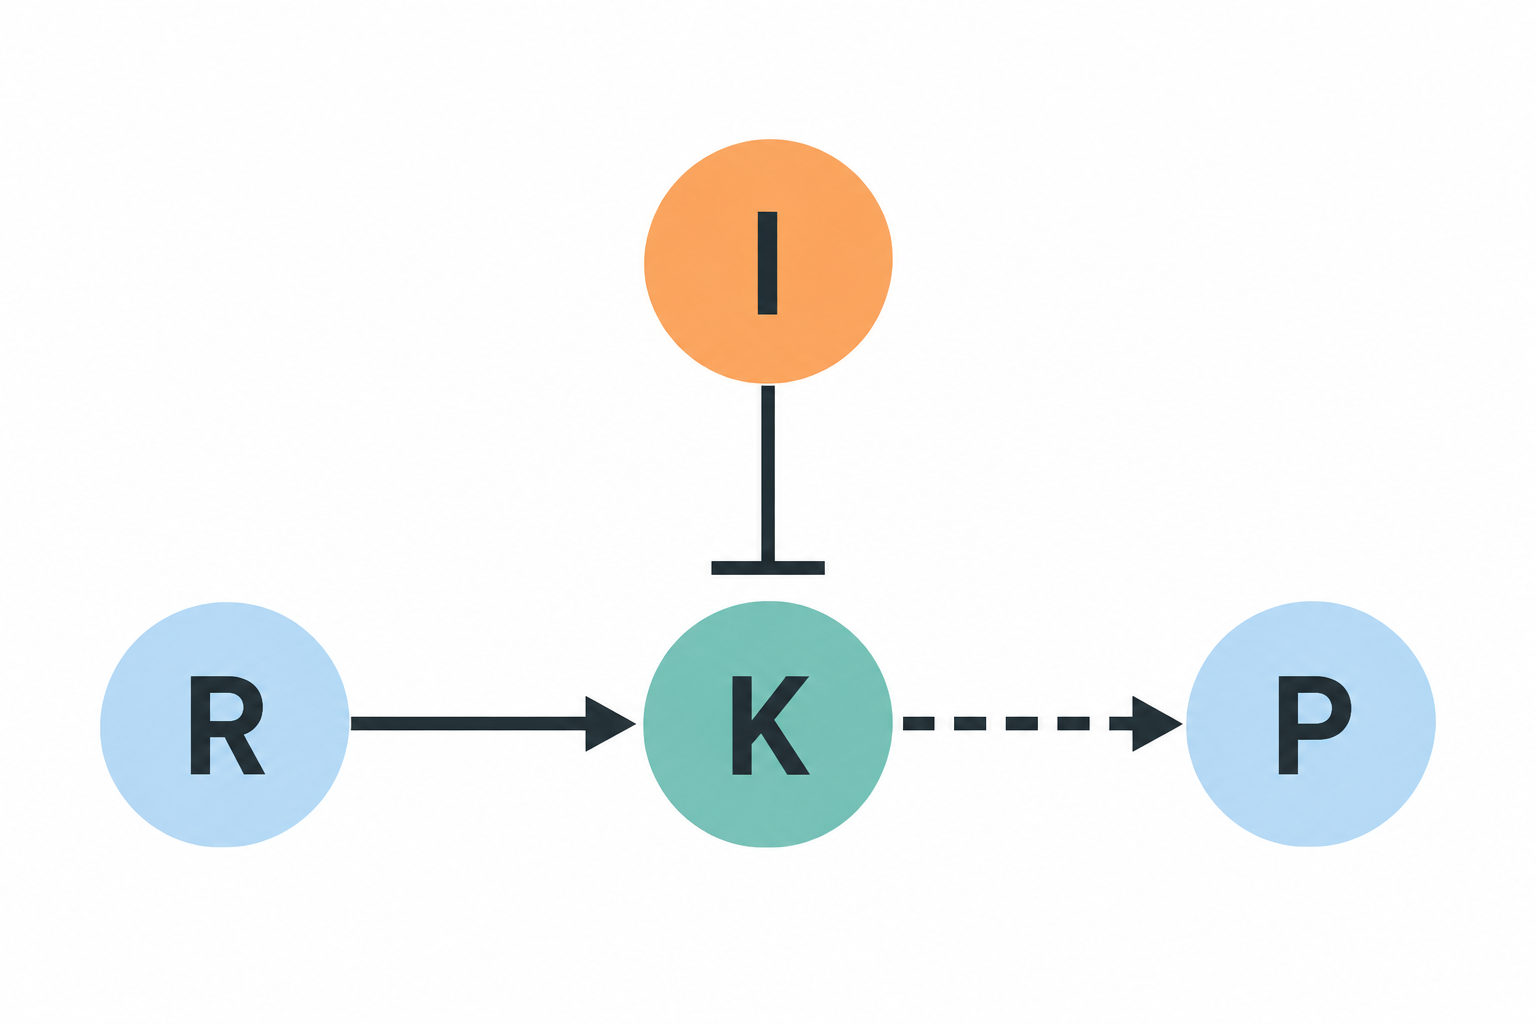
\includegraphics[width=\linewidth]{figures/mechanism-codex.png}
\caption{Codex 内置图像生成的抽象教学模型。实线箭头表示给定的激活关系，虚线箭头表示假设关系，T 形终点表示抑制。四个符号与全部关系均为教学设定，不对应真实分子或研究发现。}\label{fig:mechanism}
\end{figure}


线型和箭头没有脱离语境的万能含义。它们的意义由学科惯例、本图定义和图例共同确定。本例使用上述约定，是为了让读者区分三种关系。真实项目应采用目标学科能理解的表达，并在可能产生歧义时直接标注。

用关系表检查图时，可以逐行进行：找 R 和 K，检查方向，再找标签。之后检查 K 到 P 的线是否仍为虚线，最后确认 I 的抑制终点确实是 K。检查任务从“这图看起来对吗”变成了几个可定位的问题。

\section{为机制案例写一份可执行的输入}

在 SciDraw AI 科研绘图向导中选择“机制图与流程图”，把默认任务书替换为下面的内容，并下载一份副本。

\begin{Prompt}
【用途与读者】用于科研绘图教学，读者无需生物学背景。
【目标】让读者分辨给定关系、假设关系和抑制关系。
【材料】仅使用本任务书的抽象教学设定。
【对象】R、K、P、I；每个对象各出现一次。
【关系】
R 激活 K：实线箭头，方向 R 到 K，旁标“激活”。
K 可能影响 P：虚线箭头，方向 K 到 P，旁标“假设”。
I 抑制 K：线条终点在 K 一侧使用短横线，旁标“抑制”。
【布局】R、K、P 从左到右；I 放在 K 上方。
【视觉】白底、二维简洁图形。四个对象以标签识别。
【限制】不添加其他对象、关系、分子形态或实验结果。
【图例】解释实线、虚线与抑制线；标注“抽象教学模型”。
【验收】四个对象、三条关系、方向与标签逐项对应。
\end{Prompt}

这个输入没有要求“达到某顶级期刊水平”。它给出了更直接的质量标准：对象可辨，关系准确，假设没有被画成确定结论。颜色可以随后调整，基本关系要先站得住。

进入机制图工具后，复制这段说明到生成输入。得到候选图时，先按关系表检查，再决定是否继续修改。如果输出多了一个对象，不能只要求“整体更简洁”；应指出多出的对象，以及保留四个对象各一次的要求。

本版已用 Codex 内置图像生成制作了图 2-1，记录了完整输入与核验结果。四个对象和三条关系均符合任务书，节点仍有轻微渐变，因此它是可核对的教学候选图，不是“所有风格要求都已精确执行”的证明。该图并非 SciDraw AI 实测输出。AI 的每一次输出都具有变动性，同一段输入并不保证自动满足全部条件。

\section{为数据图写约束，要具体到列}

数据图的任务书需要从研究设计延伸到数据结构。第一章的练习只有三列，也足以说明几种常见歧义。

\texttt{sample\_id} 用来识别同一个对象；\texttt{before} 和 \texttt{after} 是该对象的两次测量。八行对应八个虚构对象，同时包含十六个观测值。对象数和测量数应分别表述。对真实研究，还需解释实验单位、重复测量和技术重复之间的关系。

下面是一段适合交给科学可视化的绘图要求：

\begin{Prompt}
读取上传的 paired-example.csv。
sample_id 是配对键；before 和 after 是两次测量，单位 a.u.。
绘制配对点线图：横轴按 before、after 排列，每个对象的两个点
由一条线相连。保留全部八个对象和原始十六个观测值。
不要把两列当成互不相关的独立样本，也不要连接不同对象。
标题为“模拟教学数据：个体前后变化”。
本练习只展示原始测量，不进行显著性检验，不添加误差线。
不得删去 SIM04 或把它的下降趋势改成上升。
\end{Prompt}

最后一句不是要求某个真实研究必须出现下降，而是本练习的核查点：文件里这个对象确实从 18 下降到 17。真实项目应依据自己的数据写核查点，不能用期望的结论倒逼图形。

输入中“不添加误差线”也只针对本次练习。其他图需要误差线时，应明确它表示标准差、标准误、置信区间或其他量，并说明计算依据。AI 无法仅凭“加上常见误差线”知道你希望传达哪种不确定性。

\section{使用 PDF 辅助时，先确认读取了什么}

论文中的信息分散在摘要、正文、图表、补充材料和方法里。上传一个 PDF 后，系统如何提取文字，会直接影响后续提示词包含哪些内容。

本次核查的 SciDraw AI PDF 辅助路径读取前五页，并从摘要或开头截取有限文本，供视觉提示词使用。它适合帮助起草研究总览，但不能据此认定整篇论文、所有图表与补充材料都已经被理解。

使用这一入口时，可先准备一份作者确认的要点：研究问题是什么，采用了哪条主要方法，准备展示哪个结果，还有哪些适用条件。将辅助生成的提示词与这份要点对照，补回遗漏，再进入绘图。若关键结果只在后文，单凭前几页输入就可能遗漏它。

在任务书来源栏记录读取范围也很有用。例如：“输入为作者整理的摘要与结果要点；PDF 辅助仅用于初稿，关键结论已对照原文确认。”这比笼统写“根据全文自动生成”准确，也便于以后重新制作。

\section{把模糊意见改写成可核对的请求}

很多重复生成并没有明确方向，只是在等待一个更合眼缘的结果。下面几种改写，可以让一次操作承担清楚的任务。

\begin{center}\small
\begin{tabularx}{\linewidth}{YY}
\toprule
\textbf{模糊表达} & \textbf{更具体的请求} \\
\midrule
画得更专业 & 将 R、K、P 水平对齐；统一标签字号；保留关系和对象数量 \\
更突出结果 & 让读者能直接比较两次测量；保留个体连线与全部观测值 \\
简化一点 & 移除装饰背景和重复说明，保留四个对象、三条关系与图例 \\
用期刊风格 & 白底，减少装饰；按已确认的文字层级与颜色角色重新排版 \\
自动补全图注 & 起草可从图中识别的描述；样本量、实验条件与统计方法由作者补充 \\
\bottomrule
\end{tabularx}
\end{center}

这些写法不保证模型绝不出错。它们的价值在于让作者能够判断要求是否执行，并定位需要重做的部分。平台当前的图片修改可能影响整张图，所以即使只要求改一个标签，也要重新检查其他对象和关系。

\section{在提交前，做一次反向阅读}

把任务书当作你第一次看到的材料，暂时不依赖脑中的研究背景，逐句寻找不完整的地方。

“处理组高于对照组”缺少哪个指标、什么条件和哪些证据。“这个步骤之后分成两组”缺少分组依据。“提高性能”缺少指标、单位和比较对象。发现这种缺口后，先补充信息，或把结论降为待确认事项。

还可以为每条拟表达的陈述建立一个小表：陈述、来源位置、拟采用的图形、需要确认的内容。真实项目中的来源可以具体到数据列、文件版本或记录页码。抽象练习则标注“教学设定”。这样做能避免来源模糊的陈述被顺手写进图中。

\section{本章练习与验收}

完成两份任务书：一份针对自己的研究，另一份使用本章抽象机制或配对数据。保留一份修改前的原始说明，再写一段修改记录，说明你补充了哪些关系、来源和验收条件。

最后逐项检查：对象能否数清，关系能否逐条核对，数据约束能否对应到列，未知信息是否仍被明确标识，最终产物是否有具体用途。

完成这些工作后，你就拥有了一个可以进入绘图阶段的输入。第三章将讨论如何把同一份任务书展开成不同构图，并用读者的理解成本来选择方案。
